\section{Methodology}

% Target ~10-15 pages. Theory + experimental methods, with references. Use block
% diagrams / flowcharts. Highlight the methodological novelty (synthetic-turbidity
% characterisation of passive-marker perception). Keep Part A / Part B parallel.

\subsection{System architecture}

\begin{figure}[H]
\centering
\begin{tikzpicture}[font=\scriptsize, >={Stealth[length=2mm]},
  box/.style={draw, rounded corners=1pt, align=center, minimum height=8mm, inner sep=3pt}]
  \node[box] (cam) {Camera\\(10~Hz)};
  \node[box, right=6mm of cam] (det) {ArUco\\detection};
  \node[box, right=6mm of det] (fus) {Spatial consensus +\\inverse-variance fusion};
  \node[box, right=6mm of fus] (kf) {Error-state\\Kalman filter};
  \node[box, below=10mm of kf] (guid) {Guidance\\(coarse standoff / fine align)};
  \node[box, left=14mm of guid] (ctl) {PBVS control +\\velocity feedforward};
  \node[box, left=14mm of ctl] (veh) {ArduSub\\+ vehicle};
  \node[box, below=8mm of ctl, dashed] (fsm) {Supervisory FSM: \textsc{idle} / \textsc{coarse} / \textsc{fine} / \textsc{docked}};
  \draw[->] (cam) -- (det);
  \draw[->] (det) -- (fus);
  \draw[->] (fus) -- (kf);
  \draw[->] (kf) -- node[right]{\tiny pose, velocity, health} (guid);
  \draw[->] (guid) -- node[above, yshift=1pt]{\tiny error} (ctl);
  \draw[->] (ctl) -- node[above, yshift=1pt]{\tiny cmd\_vel} (veh);
  \draw[dashed, ->] (veh.north) -- node[left]{\tiny camera moves with vehicle} (cam.south);
  \draw[dashed, ->] (fsm.north) -- (ctl.south);
  \draw[dashed, ->] (fsm.east) -| node[pos=0.35, below]{\tiny engage / handoff / demote} (guid.south);
\end{tikzpicture}
\caption{System architecture. Perception runs entirely in the loop; the
supervisory state machine sequences the mission and gates the controllers
on the filter's health signal. The feedback path from vehicle to camera is
the ego-motion coupling analysed in Section~\ref{sec:results-a}.}
\label{fig:arch}
\end{figure}

The system is a perception, guidance and control pipeline for the terminal stage
of docking. Perception estimates the dock pose from passive ArUco markers and
publishes a filtered pose, a dock velocity estimate, and a semantic health
signal. Guidance converts the dock pose and the vehicle pose into a body-frame
error to a target point. Control regulates that error with position-based
visual servoing (PBVS) and writes a body velocity command. A supervisory state
machine sequences the mission through \textsc{idle}, \textsc{coarse} (drive to
a standoff point on the dock entry axis), \textsc{fine} (align and advance into
the entry) and \textsc{docked}, with demotion paths on loss of the perception
signal.

PBVS was selected over image-based servoing because the marker pipeline already
produces a full metric 6-DOF pose: fusing multiple markers of known geometry
yields a calibrated dock pose, so servoing in pose space costs nothing extra
and keeps the guidance geometry (standoff points, entry axis, capture
tolerances) expressible in physical units \cite{chaumette2006visual}.

The scope boundary is the optical terminal stage: trials begin with the dock
inside the camera field of view at several metres range. Long-range
acquisition (acoustic homing or an active light cue) is assumed to have
delivered the vehicle to this point and is out of scope.

\begin{figure}[H]
\centering
\begin{tikzpicture}[font=\scriptsize, >={Stealth[length=2mm]}, node distance=16mm,
  st/.style={draw, rounded corners=3pt, align=center, minimum height=9mm, inner sep=4pt}]
  \node[st] (idle) {\textsc{idle}\\ \tiny re-arm, hold};
  \node[st, right=of idle] (coarse) {\textsc{coarse}\\ \tiny drive to standoff};
  \node[st, right=of coarse] (fine) {\textsc{fine}\\ \tiny align, advance};
  \node[st, right=of fine] (dock) {\textsc{docked}\\ \tiny disarm};
  \draw[->] (idle) -- node[above, align=center]{\tiny engage} (coarse);
  \draw[->] (coarse) -- node[above, align=center]{\tiny handoff gate:\\ \tiny pos + yaw tol,\\ \tiny velocity-matched,\\ \tiny debounced} (fine);
  \draw[->] (fine) -- node[above, align=center]{\tiny seated $\leq$ 0.10 m,\\ \tiny debounced} (dock);
  \draw[->] (fine.south) to[bend left=25] node[below, align=center]{\tiny demote: loss $>$ 2 s or range $>$ 1.5 m} (coarse.south);
  \draw[->] (coarse.north) to[bend right=30] node[above]{\tiny disengage} (idle.north);
  \draw[->] (dock.north) to[bend right=45] node[above]{\tiny disengage (re-arm on \textsc{idle} entry)} (idle.north);
\end{tikzpicture}
\caption{Docking state machine with the transition gates annotated.
Demotion paths make perception loss recoverable rather than terminal.}
\label{fig:fsm}
\end{figure}

\subsection{Part A: Docking simulation}

\subsubsection{Simulation environment}
\label{sec:method-sim}

The simulation runs ROS~2 Jazzy with Gazebo (gz-sim~8, DART physics) and an
ArduSub software-in-the-loop autopilot coupled through the ArduPilot Gazebo
plugin, using the BlueROV2 Heavy model with hydrodynamic and buoyancy plugins
from the blue-sim stack. The vehicle carries a forward camera simulated at
10~Hz. The world places a docking station 5~m ahead of the vehicle spawn
point at 1.5~m depth, carrying a printed board of nine ArUco markers
(47.5~mm to 200~mm) whose layout matches the physical board of Part~B.

Dock motion is generated by a custom Gazebo plugin that drives the dock
through a sinusoidal sway and heave of amplitude 0.1~m with a 90-degree
relative phase, producing an orbital motion representative of wave-driven
excitation of a moored structure. The period is configurable per launch
(18~s nominal; 6~s to 20~s in the envelope sweep) and the plugin publishes
the true dock pose as a ground-truth channel used only for scoring, never
by the vehicle. Mechanical capture and contact are not modelled: success
is defined at the capture envelope (Section~\ref{sec:method-experiment})
and would-be contacts are scored post hoc from ground truth.

The swept period band and amplitude are anchored to real ocean forcing.
Surface gravity waves occupy roughly 5 to 20~s: locally generated wind sea
at 5 to 8~s and swell from 8~s up to about 20~s
\cite{holthuijsen2007waves}, and the long-term mean off the New South
Wales coast, the operating context of this work, is a significant wave
height of 1.6~m at a mean period of 8~s \cite{kinsela2024nearshore}. A
submerged dock, moored or suspended \cite{guo2024dynamic}, is forced by
the wave orbital motion, whose amplitude decays with depth as $e^{-kz}$
with $k = 2\pi/L$ and deep-water wavelength
$L = gT^2/2\pi \approx 1.56\,T^2$ \cite{holthuijsen2007waves}, so
long-period swell penetrates far deeper than wind sea. Taking the
water-particle orbital excursion as a proxy for the excursion of a
compliantly moored dock, the simulated 0.1~m amplitude corresponds, in
the mean NSW sea state, to a dock at approximately 19~m depth for the
6~s period, 33~m at 8~s, 52~m at 10~s and beyond 200~m at 20~s;
shallower docks see larger amplitudes, deeper docks only the long-period
components. Sweeping 6 to 20~s at a fixed 0.1~m amplitude therefore
isolates the period dependence while keeping every cell identifiable
with a physically realistic sea state and operating depth (the
deep-water decay is conservative for the longest periods at
continental-shelf depths, where finite-depth theory retains still more
motion).

\subsubsection{Perception (simulated ArUco pipeline)}

The full perception pipeline runs in the loop; the controller never sees
ground truth. Markers are detected on the simulated camera stream and each
detection is converted to an implied dock-origin pose using the known marker
layout. A spatial-consensus test rejects outlier detections, and the
surviving markers are fused by inverse-variance weighting with a range-scaled
noise model, $\sigma = \alpha r^2 / s$ for a marker of size $s$ at range
$r$, so distant small markers contribute less than near large ones.

The fused measurement feeds a nine-state error-state Kalman filter over dock
position, dock velocity and a small-angle rotation error carried about a
reference quaternion \cite{sola2017quaternion}.
Two process-noise regimes are defined. The \emph{static} regime pins the
velocity states (zero initial velocity uncertainty and zero velocity process
noise), which is algebraically equivalent to a constant-position filter and
serves as the baseline. The \emph{sway} regime models constant-velocity
motion with a white-noise-acceleration process of density $\sigma_a$
(0.16~m/s$^2$ nominal, exposed as a parameter), enabling dock velocity
estimation and the feedforward of Section~\ref{sec:method-control}. Updates
are gated by a Mahalanobis test, the velocity state is bounded by a physical
dock-speed limit (0.2~m/s), and the filter publishes its velocity state as a
twist alongside the pose.

A health classifier maps filter state to \textsc{warming}, \textsc{healthy},
\textsc{degraded} or \textsc{stale} from the age of the last accepted
measurement and the position uncertainty: healthy requires a recent update
and position standard deviation under 0.04~m, and the estimate is declared
stale when either the measurement age exceeds 3~s or the uncertainty exceeds
a 0.15~m ceiling, so controllers hold rather than act on an unconstrained
estimate. Downstream controllers consume only this semantic signal.

\begin{figure}[H]
\centering
\begin{tikzpicture}[font=\scriptsize, >={Stealth[length=2mm]},
  box/.style={draw, rounded corners=1pt, align=center, minimum height=9mm, inner sep=3pt}]
  \node[box] (meas) {fused\\measurement};
  \node[box, right=7mm of meas] (gate) {Mahalanobis\\gate};
  \node[box, right=7mm of gate] (upd) {update\\ $[\,\delta p \;\; \delta v \;\; \delta\theta\,]$};
  \node[box, right=7mm of upd] (bound) {bounds:\\ $|v| \leq 0.2$ m/s,\\ $\sigma_p$ ceiling};
  \node[box, right=7mm of bound] (out) {pose, twist,\\health};
  \node[box, below=7mm of upd] (pred) {predict (30 Hz)\\ \emph{static}: $v$ pinned $\;|\;$ \emph{sway}: WNA $\sigma_a$};
  \draw[->] (meas) -- (gate);
  \draw[->] (gate) -- (upd);
  \draw[->] (upd) -- (bound);
  \draw[->] (bound) -- (out);
  \draw[->] (pred) -- (upd);
\end{tikzpicture}
\caption{Filter structure: the nine-state error-state filter with the two
process-noise regimes (the Part~A ablation), the measurement gate, and
the physically motivated state bounds.}
\label{fig:kf}
\end{figure}

\subsubsection{Guidance and control}
\label{sec:method-control}

Coarse approach regulates a standoff point 1~m out along the dock entry
axis with per-axis PD control, a distance-gated surge cap that bounds the
worst-case closing speed, and the autopilot in depth-hold. Handoff to fine
alignment is gated by position, boresight-offset and yaw tolerances plus a
velocity-match term (an exponentially smoothed derivative of the
standoff-relative position, threshold 0.15~m/s) sustained through a
debounce, so the handoff cannot latch at a sway zero crossing where the
position error is momentarily small while the dock moves fastest.

Fine alignment implements align-then-advance: surge toward the entry is
inhibited until lateral, vertical and yaw errors are within alignment
tolerances, with the autopilot in stabilise mode so the controller owns
depth. The seat criterion (definition of docked) is a debounced 0.10~m
range to the entry with 0.03~m lateral and vertical tolerances; the 0.10~m
value is derived from the measured sensing envelope in
Section~\ref{sec:results-a}, which shows marker visibility collapsing below
approximately 5~cm, so the seat is confirmed where vision is still reliable
and the final centimetres are delegated to the capture mechanism assumed by
the envelope definition.

Both controllers accept a dock-velocity feedforward built from the filter
velocity state rotated into the body frame. The feedforward is clamped
dock-relatively (the feedback term retains its full authority budget and the
feedforward is limited separately at 0.25~m/s), scaled by a distance-gated
authority ramp (zero beyond 1.5~m from the standoff, full inside 0.3~m),
and converted from physical velocity to command units by a gain of 0.6
identified from the plant response: the command channel is effort-like, with
a measured steady gain of 1.3 to 1.6 and approximately 240~ms of lag between
command and vehicle velocity. In the static filter regime the velocity
estimate is identically zero, so the feedforward vanishes and the system
reduces exactly to the baseline controller; this is the ablation used
throughout Part~A.

\begin{figure}[H]
\centering
\begin{tikzpicture}[font=\scriptsize, >={Stealth[length=2mm]}, scale=1.15]
  % dock cage (top view), entry faces left
  \fill[gray!30] (8.0,-0.75) rectangle (9.6,0.75);
  \fill[white] (8.0,-0.55) rectangle (9.4,0.55);
  \draw[thick] (8.0,-0.75) rectangle (9.6,0.75);
  \draw[thick] (8.0,-0.55) rectangle (9.4,0.55);
  \node at (8.8,1.05) {dock (top view)};
  % entry axis
  \draw[dashed] (0.2,0) -- (8.0,0);
  \node at (5.2,0.25) {\tiny entry axis};
  % blackout zone
  \fill[red!12] (7.6,-0.6) rectangle (8.0,0.6);
  \node[red!60!black, align=center] at (6.3,-1.45) {\tiny vision blackout $<$ 0.05 m};
  \draw[red!60!black, ->] (6.7,-1.3) -- (7.8,-0.5);
  % entry plane + aperture
  \draw[<->] (8.1,-0.55) -- (8.1,0.55);
  \node[align=center] at (9.3,-1.15) {\tiny aperture\\ \tiny $\pm$0.15 m};
  \draw[->] (9.0,-0.98) -- (8.15,-0.4);
  % seat point
  \draw[thick] (7.2,-0.15) -- (7.2,0.15);
  \node[align=center] at (6.1,0.95) {\tiny seat: 0.10 m,\\ \tiny $\pm$0.03 m lateral};
  \draw[->] (6.4,0.72) -- (7.15,0.2);
  % standoff
  \node at (3.4,0) {$\times$};
  \node[align=center] at (3.4,0.55) {\tiny standoff point\\ \tiny (coarse target)};
  % vehicle
  \draw[fill=gray!15] (1.0,0.25) -- (2.0,0) -- (1.0,-0.25) -- cycle;
  \node at (1.3,0) {\tiny ROV};
  \draw[->] (2.1,0) -- (3.15,0);
  % distance annotations
  \draw[|<->|] (3.4,-0.9) -- (8.0,-0.9);
  \node at (5.0,-1.1) {\tiny 1.0 m (not to scale)};
\end{tikzpicture}
\caption{Terminal docking geometry (top view, not to scale): the coarse
standoff point, the fine-alignment entry axis, the 0.15~m scoring
aperture, the 0.10~m seat criterion, and the close-range vision blackout
that motivates seating before the blind zone.}
\label{fig:geometry}
\end{figure}

\subsubsection{Experimental method}
\label{sec:method-experiment}

Trials are executed by an unattended harness that launches the full stack,
waits for the filter to initialise and the autopilot mode to settle,
engages the state machine, records a curated set of topics, polls for the
docked state with a timeout, and tears the stack down between trials.
Recording runs in a low-impact configuration after measurements showed
recorder load itself degrading the perception cadence it was capturing.

The envelope experiment sweeps filter regime (\emph{static} baseline versus
\emph{sway} method) by dock sway period $\{20, 16, 12, 10, 8, 6\}$~s with
three sway start phases per cell ($n{=}3$) plus a static-dock sanity cell per
regime, 38 trials per sweep. Scoring uses the ground-truth channel only.
Each trial receives one of three outcomes: \textsc{clean dock} (docked with
no pre-latch off-aperture crossing), \textsc{contact} (the vehicle volume
crossed the dock structure envelope more than 0.15~m from the calibrated
entry axis before the seat latched; the trial is censored at that instant
because subsequent motion traverses space a physical dock would deny), or
\textsc{no dock}. Crossing the entry plane inside the aperture is normal
insertion and is not a contact. The aperture radius is a stated assumption
standing in for a capture funnel; the two observed populations (centred
insertions at 0.003 to 0.05~m offset versus misses at 0.17~m and beyond)
are far from the boundary, so conclusions are insensitive to its exact
value. The full sweep was run twice, on two hosts (real-time factors 0.6
and 1.0) and two filter revisions, to check that conclusions do not depend
on load, hardware or incidental tuning.

\subsection{Part B: Real-CV validation}
\label{sec:method-partb}

\subsubsection{Marker target and its as-printed geometry}

The target uses the original ArUco dictionary (5$\times$5 payload) with the
dock's marker set: two 155.64~mm markers (IDs 201, 202), one 77.82~mm (301),
four 46.69~mm (302 to 305) and two 36.96~mm (401, 402), printed across three
A4 sheets taped to a rigid panel. The as-printed geometry was estimated from
the data rather than assumed: a size-weighted least-squares fit over all nine
markers (residuals under 0.4~mm) shows the sheets were printed at 95.9\% of
nominal scale, so the analysis uses the measured black-square sides (149.4,
74.7, 44.4 and 35.6~mm) throughout. The fit is corroborated independently by
the 201-to-202 baseline, which matches two butted A4 pages plus millimetres
of tape gap only under the corrected scale; using nominal sizes would
silently inflate every derived range by 4.1\%. The as-measured layout is
shown in Figure~\ref{fig:board}.

\begin{figure}[H]
    \centering
    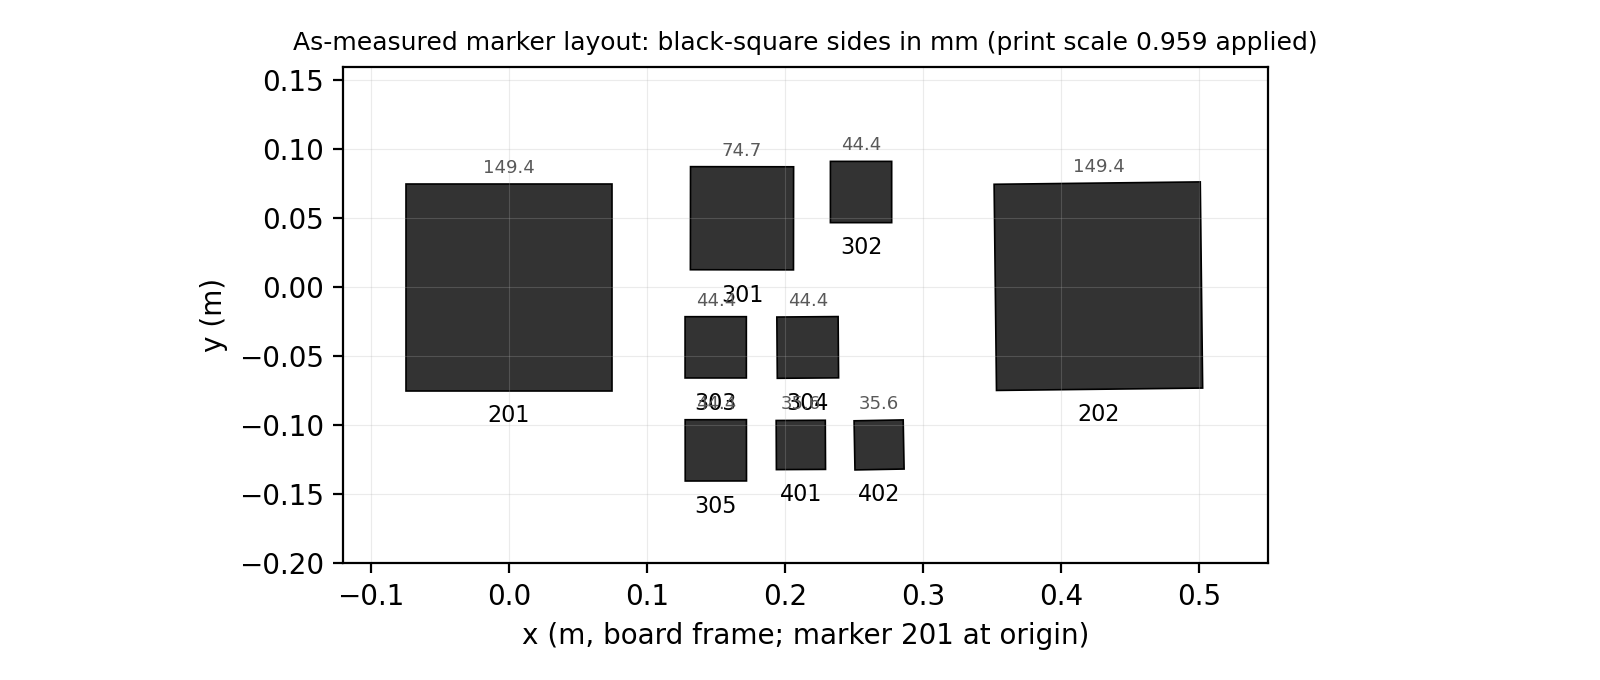
\includegraphics[width=0.85\textwidth]{Figures/board_layout.png}
    \caption{As-measured marker layout in the board frame, positions and
    black-square sides estimated from the data with the 0.959 print scale
    applied. The four size groups placed at a common range are the
    marker-size lever of the experiment.}
    \label{fig:board}
\end{figure}

\subsubsection{Capture setup}

Data was captured in a single pool session with a ZED stereo camera, of
which only the left, rectified stream was recorded (960$\times$540 at
nominal 15~Hz), giving a monocular ArUco problem; images, camera info and
the ZED IMU were logged. Two runs were
recorded: an on-axis walk-back (677 frames at an effective 2.5~Hz over
271~s) and an oblique walk-back from roughly 4~m of lateral offset (737
frames over 85~s, with about 42\% of frames dropped in bursts by disk
bandwidth; the two runs are therefore analysed separately and never
pooled). The vehicle was hand-held and paced backwards from the board to
beyond the detection limit, with a yaw turn at each step.

Camera intrinsics are the shipped in-air factory rectification
($f_x{=}f_y{=}797.5$, zero distortion on the rectified stream). The
in-water validity of this choice was tested by a joint bundle adjustment
over 1400 marker observations in 317 frames, solving for underwater focal
lengths, the coplanar board layout and per-frame poses with scale pinned by
the ruler-measured marker sizes: the aspect ratio solves to
$f_y/f_x = 0.996$ and the isotropic optimum is only 1.9\% better than the
in-air value, while the flat-port refraction correction of $1.333\times$
is rejected outright (44\% worse residual). The shipped intrinsics are
therefore used unchanged, and all metric ranges carry an approximately
$\pm$10\% scale uncertainty from the focal length, which dominates the
error budget. For this reason the primary independent variable throughout
Part~B is the calibration-free \emph{apparent marker size in pixels};
metric range is derived and reported with its uncertainty.

\subsubsection{Experiment design}

The two walk-backs sweep range continuously from about 0.6~m to beyond the
detection limit, and marker size is swept \emph{by construction}: four size
groups (149.4 down to 35.6~mm, a 4.2$\times$ lever) are present on the
board simultaneously, so every frame samples all sizes at a common range
and water condition. Viewing angle was not controlled: the on-axis run has
a median marker incidence of 13$^\circ$ and the oblique run 58$^\circ$,
two disconnected regimes confounded with range and marker size, so no
detection-versus-angle curve is reported.

No external ground truth exists (no tape or survey range, and vehicle
odometry was not recorded); scale is anchored solely by the ruler-measured
marker sizes and attitude solely by an IMU gravity check. Detection is
scored per marker-frame trial against apparent-size bins with a minimum of
ten trials per bin and Wilson confidence intervals (2551 trials on-axis,
950 oblique). Maximum detection range is established uncensored: the
on-axis walk continued for a further 79~s (about 3~m) beyond the last
detection with zero detections, and two independent end-of-run estimates
(walk-back rate extrapolation and board apparent width in the final frame)
agree at 7.8 to 8.1~m, so range limits below are detection failures, not
end-of-data artefacts.

\subsubsection{Turbidity measurement and synthetic degradation}

Water attenuation was measured photometrically from the target itself,
without dosing or a turbidity meter. A black patch (marker border) and a
white patch (surrounding sheet) at the same range share an identical
veiling-light term in the image formation model
$I = J e^{-\beta d} + B(1 - e^{-\beta d})$, so their difference is free of
$B$: $\mathrm{contrast}(d) = (J_w - J_b)\,e^{-\beta d}$, and $\beta$ is a
straight-line fit in log space. Two corrections proved load-bearing: an
instrument-response correction $k$(apparent~px), measured at fixed range so
it is independent of $\beta$, without which small (hence distant-looking)
markers read up to 18\% low and the bias imitates attenuation; and
per-marker intercepts, since the three sheets sit under different local
lighting. The underlying image formation model is the standard
attenuation-plus-veiling form \cite{jaffe1990computer}.

Higher turbidity than the pool's was synthesised by re-attenuating each
real frame in place: $I' = B + (I - B)\,e^{-\Delta\beta\, d(x)}$ per
channel and per pixel, with the per-pixel range $d(x)$ taken from the
board-plane pose and $\Delta\beta = m\,\beta$ for multipliers
$m \in \{0, 0.25, 0.5, 1, 1.5, 2, 3, 4, 6, 8\}$, where $m{=}0$ reproduces
the real frame. Results are reported against total optical depth
$\tau = (1{+}m)\,\beta d$ rather than named water types: range enters the
model only as the product $\beta d$, so any uniform scale error in $d$ is
absorbed into $\beta$, making the $\tau$ axis immune to the $\pm$10\%
range uncertainty and portable across waters and cameras. The synthesis
adds no scattering blur, so any benefit a contrast-enhancing preprocessor
shows on synthesised frames is an upper bound. The full chain is
summarised in Figure~\ref{fig:turbpipe}.

\begin{figure}[H]
\centering
\begin{tikzpicture}[font=\scriptsize, >={Stealth[length=2mm]},
  box/.style={draw, rounded corners=1pt, align=center, minimum height=9mm, inner sep=3pt}]
  \node[box] (frame) {frame};
  \node[box, right=6mm of frame] (warp) {canonical\\marker warp};
  \node[box, right=6mm of warp] (patch) {black ring /\\white surround};
  \node[box, right=6mm of patch] (contrast) {$B$-free contrast\\$(J_w{-}J_b)e^{-\beta d}$};
  \node[box, right=6mm of contrast] (corr) {$k(\mathrm{px})$ +\\fixed effects};
  \node[box, right=6mm of corr] (beta) {$\beta$ per\\channel};
  \node[box, below=8mm of beta] (synth) {re-attenuate:\\$I' = B + (I{-}B)e^{-m\beta d(x)}$};
  \node[box, left=6mm of synth] (sweep) {detection sweep\\(2551 trials $\times$ 10 levels)};
  \node[box, left=6mm of sweep] (env) {envelope:\\rate(px, $\tau$), sizing rule};
  \draw[->] (frame) -- (warp);
  \draw[->] (warp) -- (patch);
  \draw[->] (patch) -- (contrast);
  \draw[->] (contrast) -- (corr);
  \draw[->] (corr) -- (beta);
  \draw[->] (beta) -- (synth);
  \draw[->] (synth) -- (sweep);
  \draw[->] (sweep) -- (env);
\end{tikzpicture}
\caption{Turbidity processing: the top row measures the water's
attenuation from the target itself via the veiling-free contrast; the
bottom row stresses the same real frames to higher optical depth and maps
the detection envelope.}
\label{fig:turbpipe}
\end{figure}

\subsubsection{Detection pipeline and metrics}

Detection uses OpenCV~4.10 with the current \texttt{ArucoDetector} API,
subpixel corner refinement, and \texttt{adaptiveThreshConstant} lowered
from the default 7 to 3, the best of a grid over $\{3, 5, 7\}$ scored at
the highest synthesised turbidity (selected without a holdout, so its
reported rate is an optimistic bound). Single-marker pose, the quantity
under test, uses planar PnP (IPPE square); the reference for
self-consistency is a multi-marker board PnP computed leave-one-out, with
the marker under test excluded from its own reference. Off-board IDs are
deliberately not filtered so the misidentification rate remains
measurable. Reported metrics are detection rate per apparent-size bin and
per derived-range bin, uncensored maximum detection range per marker,
single-marker translation and rotation deviation from the board reference
(self-consistency, not accuracy, since no ground truth exists),
misidentification rate, and an IMU gravity check as the sole
camera-independent attitude validation.
